\section{Solving Identification with a Control Function}
\label{sec:controlfun}
If your goal is to estimate CM effects, and you could control for unobserved selection terms $U_{0,i}, U_{1,i}$, then you would.
This ideal example would yield unbiased estimates.
% Alas, $U_i$ is by definition unobserved.
The control function method takes this insight seriously, providing conditions to model the implied unobserved confounding by $U_{0,i}, U_{1,i}$, and then control for it.\footnote{
    This section does not improve on the control function approach, instead only noting its utility to solve the identification problem of CM in a natural experiment setting.
}

Suppose the vector of control variables $\vec X_i$ has at least two entries;
denote $\vec X_i^{\text{IV}}$ as one entry in the vector, and $\vec X_i^-$ as the remaining rows.
\begin{definition}
    \label{dfn:controlfun-assumptions}
    Control function assumptions.
    \begin{align}
        \label{eqn:firststage-monotonicity}
        &\Probgiven{ D_i(1) \geq D_i(0) }{\vec X_i} = 1    \\
        \label{eqn:controlfun-iv}
        &\vec X_i^{\text{IV}} \text{ has the property }
        \partialdiff[\mu(\vec X_i)]{\vec X_i^{\text{IV}}} = 0 < \partialdiff[D_i(z')]{\vec X_i^{\text{IV}}}, \textnormal{ for } z' = 0, 1.
    \end{align}
\end{definition}
Assumption \ref{dfn:controlfun-assumptions}\eqref{eqn:firststage-monotonicity} is the (conditional) monotonicity assumption \citep{imbens1994identification}, which is untestable but acceptable in many empirical applications.
Assumption \ref{dfn:controlfun-assumptions}\eqref{eqn:controlfun-iv} is assuming that an instrument exists, which satisfies an exclusion restriction (i.e., not impacting mediator gains $\mu$), and has a non-zero influence on the mediator (i.e., strong first-stage).
The exclusion restriction is untestable, and must be guided by domain-specific knowledge; strength of the first-stage is testable, and must be justified with data by methods common in the instrumental variables literature.

Write $K_i$ for the error in predicting the mediator with observed data, as a function of the instrument $\vec X_i^{\text{IV}}$ and remaining controls $\vec X_i^-$.
$K_i$ serves as the control function in this setting.
\[ K_i = D_i - \Egiven{D_i}{Z_i, \vec X_i^{\text{IV}}, \vec X_i^-} \]

\begin{theorem}
    \label{thm:controlfun}
    If \ref{dfn:controlfun-assumptions}\eqref{eqn:firststage-monotonicity} and \ref{dfn:controlfun-assumptions}\eqref{eqn:controlfun-iv} hold, then the average potential outcomes are identified by a control function approach.
    \[ \Egiven{Y_i}{Z_i = z', D_i = d', \vec X_i^-, K_i}
        = \Egiven{Y_i(z', d')}{\vec X_i^-, K_i}
        , \;\; \text{ for } z', d' = 0,1. \]
\end{theorem}
\begin{proof}
    Special case of \citet[Theorem~1]{imbens2009identification}; see \autoref{appendix:controlfun-proof}.
\end{proof}

Assumption \ref{dfn:controlfun-assumptions}\eqref{eqn:firststage-monotonicity} guarantees that mediator $D_i(.)$ can be represented by a selection model \citep{vytlacil2002independence}, and \ref{dfn:controlfun-assumptions}\eqref{eqn:controlfun-iv} pins down a control function to identify the selection model.
The approach exploits the fact that the bias terms, coming from correlated the errors in \autoref{sec:regression}, can be estimated in a first-stage regression and included as controls in the second-stage.

If the underlying selection model had been a Roy model, the control function approach captures the unobserved benefits to taking mediator (independent of observed controls), and thus driving take-up of the mediator.
By incorporating the selection term derived from the first-stage model, the approach adjusts for the unobserved confounding from unobserved gains.
By contrast, assuming the mediator was ignorable would have been assuming that there are no unobserved benefits to the mediator take-up, so that there is no bias in the second-stage to account for.

The instrument is key to avoid distributional assumptions on the unobserved errors terms.
In the Roy model, the exclusion restriction can be satisfied in one key way: having an instrument for cost of mediator take up $\mu_C$.
If the instrument $\vec X_i^{\text{IV}}$ enters the cost function $\mu_C$, and not the benefits function $\mu$, then it satisfies the exclusion restriction.
In an applied world, $\vec X_i^{\text{IV}}$ can be data that explain cost differences in taking $D_i$, unrelated to other demographic information.
If a researcher is looking into higher education as a proposed mediator, then data which explains different costs of attending university (unrelated to education gains) can serve this role.
This is the logic behind the \cite{card1993using} distance-instrument, and can be extended to a CM setting with education as the mediator.

%\textbf{Senan note:} Needs a step involving re-weighting to the D(z) compliers in the LAIE estimation.
% This is done by estimating the second-stage with Abadie (2003) re-weighting.

\subsection{Estimation}
In practice, the approach relies on estimating the control function $K_i$, then including this in the second-stage as a control, and accounting for the estimation error for these in the standard errors.
These reliances come with major concerns.
First, it is imperative that the control function is estimated correctly, so it is necessary to employ a non-parametric approach to estimate the first-stage.
Second, the error terms enters the outcome equation \eqref{eqn:parametric-secondstage} linearly, but is an unknown function (possibly non-linear) of the control function; thus, the second-stage must be estimated semi-parametrically.\footnote{
    In practice this can be done by adding a polynomial for the estimated control function into the outcome regression, or a splines approach, etc. 
}
Lastly, the standard errors must account for estimation uncertainty in the above two non-parametric steps.

These concerns are worth noting, because non-parametric regression is computationally demanding, and requires large samples for estimator convergence. 
Furthermore, these are estimated in two steps, so that the concerns are of greater importance.
Otherwise, small sample bias properties could even dominate the bias terms identified in \autoref{thm:selection-bias}.\footnote{
    See \cite[Section~6]{imbens2009identification} for a full discussion of the asymptotic theory of a control function estimator.
}
It is beyond the scope of this paper to develop the optimal procedure here, but this concern is incredibly important to keep in mind.
% Senan note: furture direction, with a real econometrician co-author?
For applied research aiming to estimate CM effects, the control function method is only appropriate in extremely large sample sizes, such as applications using administrative sources or biobanks.

With these concerns in mind, I propose the following method to estimate CM effects with a control function approach:
\begin{enumerate}
    \item Estimate the first-stage, $\Egiven{D_i}{Z_i, \vec X_i^{\text{IV}}, \vec X_i^-}$ with a non-parametric estimator (e.g., a probability forest, or fully interacted OLS specification).
    \item Calculate estimates of the control function, $\hat K_i = D_i - \hat{\mathbb E} \left[D_i \middle\vert Z_i, \vec X_i^{\text{IV}}, \vec X_i^- \right]$.
    \item Estimate the second-stage with OLS (including an interaction term between $Z_i$ and $D_i$), and a semi-parametric regressor of the control function.
    \[ \mathbb{E} \left[Y_i \middle\vert Z_i, D_i, \vec X_i^-, \hat K_i \right]
    = \beta D_i + \gamma Z_i + \delta Z_i D_i + l\left( \hat K_i \right) \]
    $l(.)$ is a semi-parametric nuisance function, so can be approximated with a spline specification, for example.
    \item Calculate the ADE and AIE estimates.
    \begin{align*}
        \hat{\text{ADE}} &= \; \E{
            \hat{\mathbb{E}} \left[ Y_i \middle\vert Z_i = 1, D_i, \vec X_i^-, \hat K_i \right]
            - \hat{\mathbb{E}} \left[ Y_i \middle\vert Z_i = 0, D_i, \vec X_i^-, \hat K_i \right]} \\
        \hat{\text{AIE}} &= \; \mathbb E \left[ \begin{aligned} &\left(
            \hat{\mathbb{E}} \left[D_i \middle\vert Z_i = 1, \vec X_i^{\text{IV}}, \vec X_i^-\right]
            - \hat{\mathbb{E}} \left[D_i \middle\vert Z_i = 1, \vec X_i^{\text{IV}}, \vec X_i^-\right] \right) \\
            &\times \left(
                \hat{\mathbb{E}} \left[ Y_i \middle\vert Z_i, D_i = 1, \vec X_i^-, \hat K_i \right]
            - \hat{\mathbb{E}} \left[ Y_i \middle\vert Z_i, D_i = 0, \vec X_i^-, \hat K_i \right]
            \right) \end{aligned} \right]
    \end{align*}
    \item Bootstrap across steps 1 through 4, to calculate standard errors.
\end{enumerate}

\subsection{Simulation Evidence}
The following simulation gives an example to show how this method works in practice.
Suppose data observed to the researcher $Z_i, D_i, Y_i, \vec X_i$ are drawn from the following data generating processes, for $i = 1, \hdots, N$.
\begin{align*}
    Z_i \sim \text{Binom}\left(0.5 \right),
    \;\; \vec X_i^- \sim N(4, 1),
    \;\; \vec X_i^{\text{IV}} \sim \text{Binom}\left( 0.5 \right), \\
    \left[ U_{0,i}, U_{1,i} \right]' \sim
    \text{BivariateNormal}\left( 0, 0, \sigma_0, \sigma_1, \rho \right),
    \;\; U_{C,i} \sim N(0, 0.25).
\end{align*}
$N = 10,000$ allows the large sample properties of the approach to operate; indeed, smaller sample sizes may not.

Suppose each $i$ chooses to take mediator $D_i$ based on the costs and benefits (i.e., a Roy model), with following definitions for each $z', d' = 0, 1$.
\begin{align*}
    \mu_{d'}\left(z' ; \vec X_i \right) = \vec X_i^- + \left( z' + d' + z' d' \right),
    \;\; \mu_{C}\left(z' ; \vec X_i \right) = 3z' + \vec X_i^- - \vec X_i^{\text{IV}}.
\end{align*}
Following \autoref{sec:selection}, these data have the following outcome equations:
\begin{align*}
    D_i &= \indicator{-3Z_i - \vec X_i^{\text{IV}} + \vec X_i^- \geq U_{0,i} - U_{1,i}},  \\
    Y_i &= Z_i + D_i + Z_i D_i + \vec X_i^-
        + \left( 1 - D_i \right) U_{0,i} + D_i U_{1,i}.
\end{align*}
In this setting the error terms $U_{i, 0}, U_{i, 1}$ determine the bias in OLS estimates of the ADE and AIE, so the bias varies for different values of the DGP parameters $\rho \in [-1, 1]$ and $\sigma_0, \sigma_1 \geq 0$.

% \textbf{To-do:} write the formula for main confounders, $\E{U_{0,i}}{D_i = 0}$ and $\E{U_{1,i}}{D_i = 1}$, which are the bias terms, and how they depend on $\rho, \sigma_0, \sigma_1$.

\begin{figure}[h!]
    \caption{OLS versus Control Function Estimates of CM Effects.}
    \begin{subfigure}[c]{0.475\textwidth}
        \centering
        \caption{ADE.}
        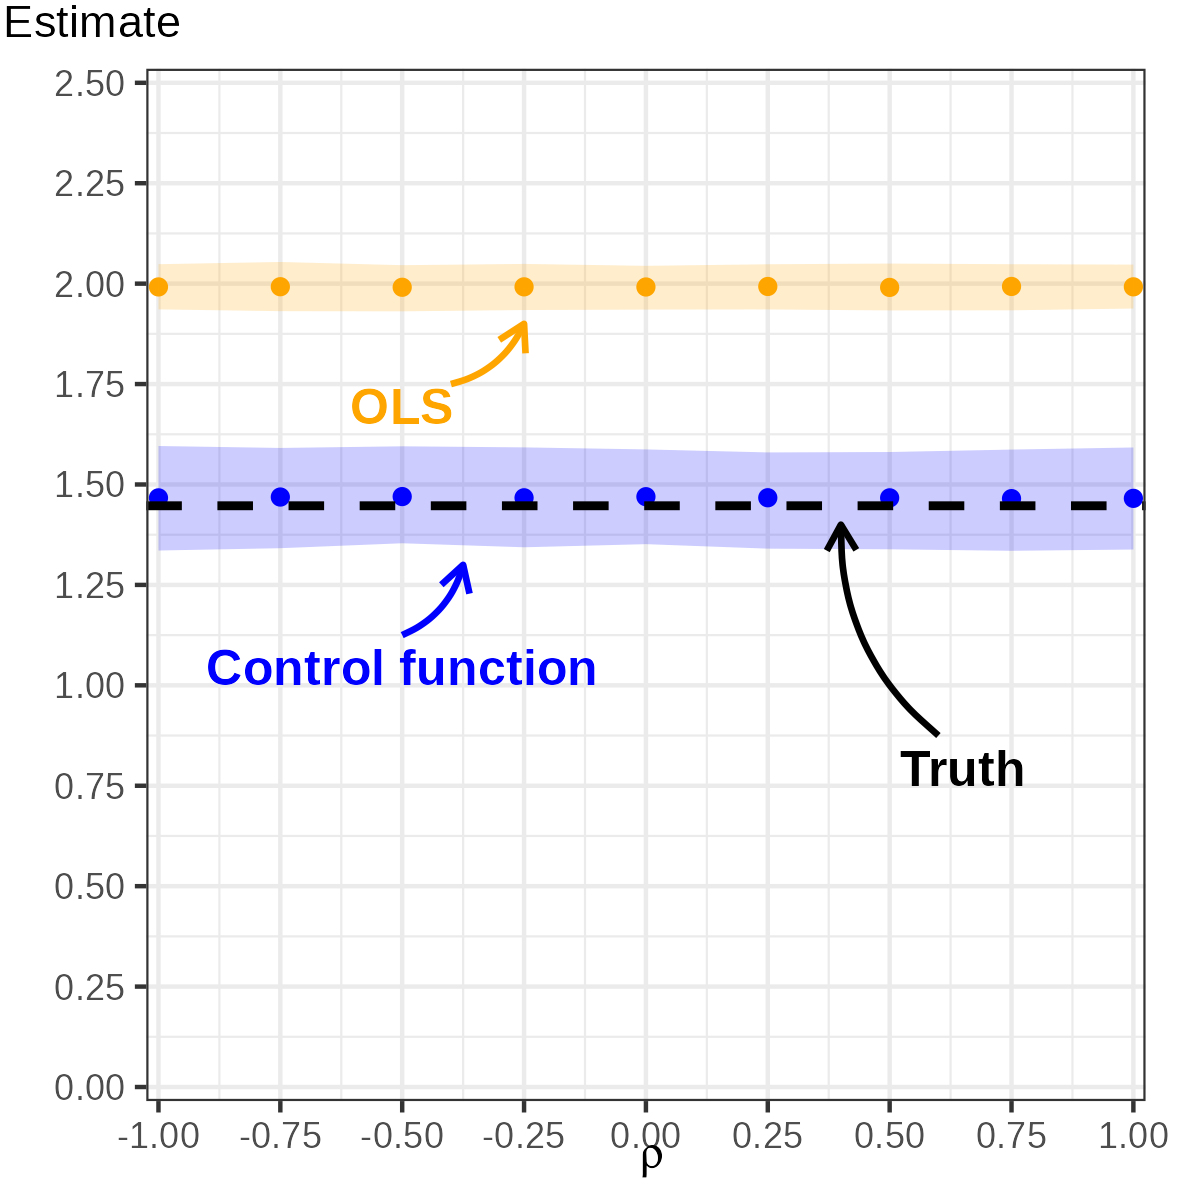
\includegraphics[width=\textwidth]{
            ../programs/simulations/sim-output/rho-directeffect-bias.png}
    \end{subfigure}
    \begin{subfigure}[c]{0.475\textwidth}
        \centering
        \caption{AIE.}
        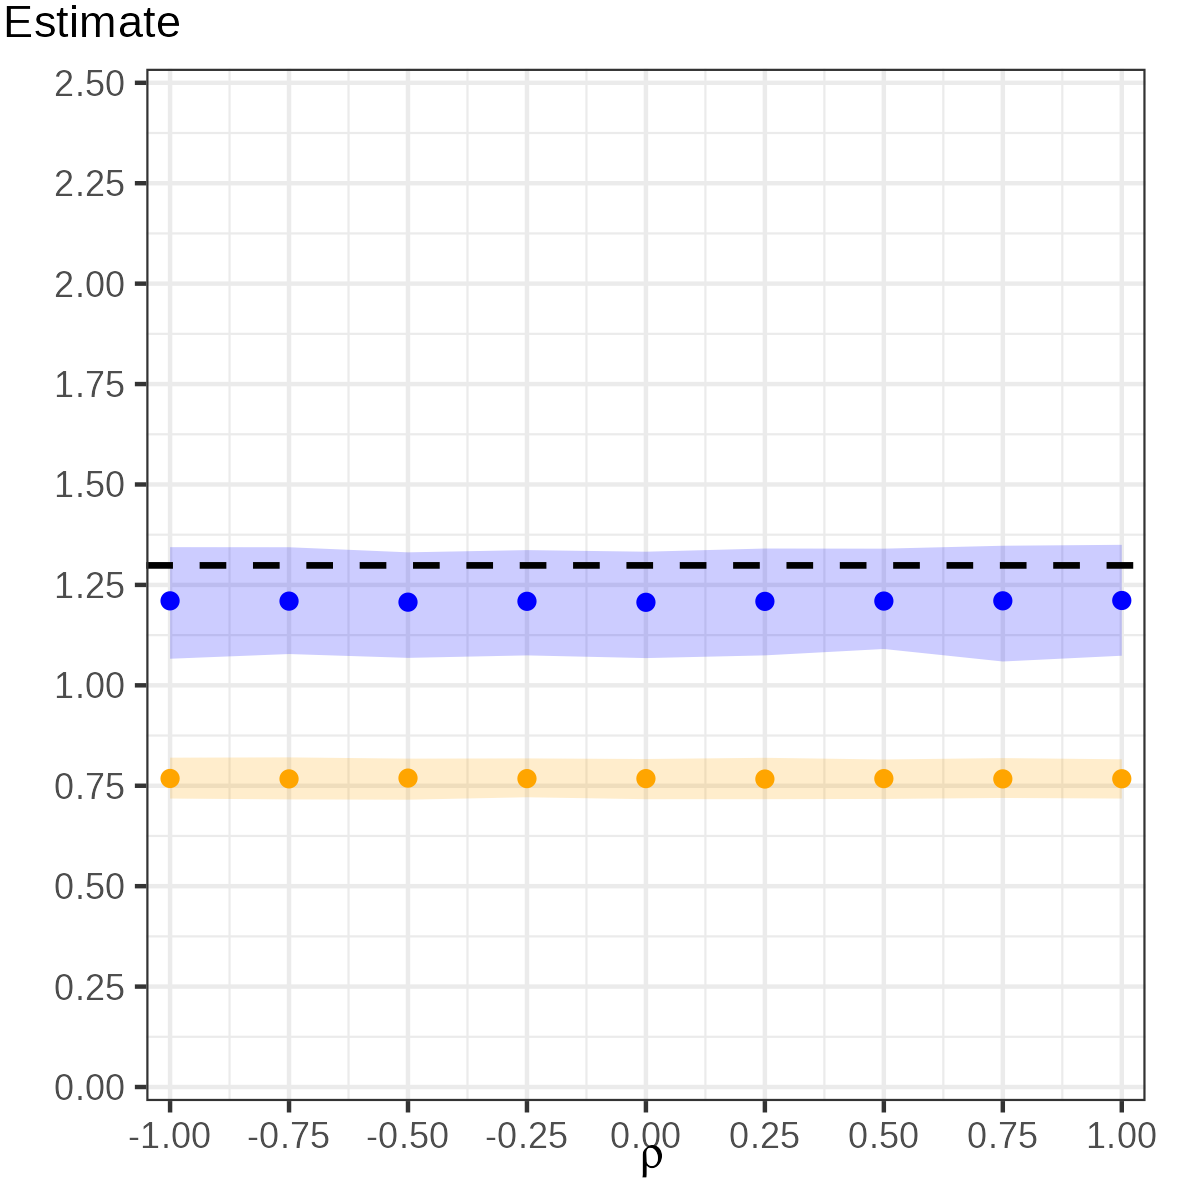
\includegraphics[width=\textwidth]{
            ../programs/simulations/sim-output/rho-indirecteffect-bias.png}
    \end{subfigure}
    \label{fig:rho-bias}
    \justify
    \footnotesize    
    \textbf{Note:}
    These figures show the OLS and control function estimates of the ADE and AIE, for $N = 10,000$ sample size.
    The black dashed line is the true value, points are points estimates from data simulated with a given $\rho$ value and $\sigma_0 = 1, \sigma_1 = 2$, and shaded regions are the 95\% confidence intervals.
    Orange are the OLS estimates, blue the control function approach described herein.
\end{figure}

\autoref{fig:rho-bias} shows the control function estimates against estimates calculated by standard OLS, showing 95\% confidence intervals calculated from bootstrapped standard errors (from 1,000 bootstrap replications).
The OLS approach implicitly asssumes that the mediator is ignorable (when it is not), so its point estimates over and under-estimate the ADE and AIE, respectively; the distance between the OLS estimates and the true values are the underlying bias terms derived in \autoref{thm:selection-bias}.
The control function approach improves on OLS estimates by correcting for the bias terms, with confidence regions overlapping the true values.\footnote{
    The code behind this simulation estimates the first-stage with an interacted OLS specification, and splines included for the continuous regression.
    The second-stage is an OLS specification, with estimated control function included (with splines) as a linear control.
}
This correction was not free: the standard errors are significantly greater in a control function approach than OLS, and exhibit small sample bias (for reasons mentioned above).
In this manner, this simulation shows the pros and cons of using the control function approach to estimating CM effects in practice.
